\documentclass[11pt]{article}
\usepackage[utf8]{inputenc}

\usepackage{latexsym}
\usepackage{amssymb,amsmath}
\usepackage{graphicx}
\usepackage{sgame}
\usepackage{xcolor}
\usepackage{authblk}

%\usepackage{indentfirst}
\usepackage[toc,page]{appendix}
\renewcommand{\appendixname}{Appendix}
\renewcommand{\appendixtocname}{Appendix}
\renewcommand{\appendixpagename}{Appendix}

\usepackage[hidelinks]{hyperref}
\usepackage{empheq}
\usepackage{blkarray}
\usepackage{cancel}
\usepackage{enumerate}
\usepackage{times}
\usepackage{array}
\usepackage{lscape}
\usepackage{setspace}

\usepackage[margin=1in]{geometry}
\newcommand{\newword}[1]{\textbf{\emph{#1}}}

%Arrows
\newcommand{\into}{\hookrightarrow}
\newcommand{\onto}{\twoheadrightarrow}

%Macros
\newcommand{\isom}{\cong} %The isomorphism symbol
\newcommand{\union}{\cup}
\newcommand{\intersection}{\cap}
\newcommand{\bigunion}{\bigcup}
\newcommand{\bigintersection}{\bigcap}
\newcommand{\disjointunion}{\sqcup}
\newcommand{\bigdisjointunion}{\bigsqcup}

\newcommand\numberthis{\addtocounter{equation}{1}\tag{\theequation}}

%Some multiletter functions
\DeclareMathOperator{\Hom}{Hom}
\DeclareMathOperator{\Ext}{Ext}
\DeclareMathOperator{\End}{End}
\DeclareMathOperator{\Tor}{Tor}
\DeclareMathOperator{\Ker}{Ker}
\DeclareMathOperator{\CoKer}{CoKer}
\DeclareMathOperator{\Spec}{Spec}
\DeclareMathOperator{\Proj}{Proj}
\renewcommand{\Im}{\mathop{\mathrm{Im}}}
%Their calligraphic versions; use these for the sheaf constructions
\DeclareMathOperator{\HHom}{\mathcal{H} \textit{om}}
\DeclareMathOperator{\EExt}{\mathcal{E} \textit{xt}}
\DeclareMathOperator{\EEnd}{\mathcal{E} \textit{nd}}
\DeclareMathOperator{\TTor}{\mathcal{T} \textit{or}}
\DeclareMathOperator{\KKer}{\mathcal{K}\textit{er}}
\DeclareMathOperator{\CCoKer}{\mathcal{C} \textit{o}\mathcal{K} \textit{er}}
\newcommand{\IIm}{\mathop{\mathcal{I} \textit{m}}}
\newcommand{\ccH}{\mathscr{H}} %The very curly H

\DeclareMathOperator{\sss}{\mathrm{sunny}}
\DeclareMathOperator{\rrr}{\mathrm{rainy}}
\DeclareMathOperator{\hhh}{\mathrm{hot}}
\DeclareMathOperator{\ccc}{\mathrm{cold}}


%This makes alternating tensors look right in displayed equations
\newcommand{\Alt}{\bigwedge\nolimits}

%Blackboard bold letters

\renewcommand{\AA}{\mathbb{A}}
\newcommand{\BB}{\mathbb{B}}
\newcommand{\CC}{\mathbb{C}}
\newcommand{\DD}{\mathbb{D}}
\newcommand{\EE}{\mathbb{E}}
\newcommand{\FF}{\mathbb{F}}
\newcommand{\GG}{\mathbb{G}}
\newcommand{\HH}{\mathbb{H}}
\newcommand{\II}{\mathbb{I}}
\newcommand{\JJ}{\mathbb{J}}
\newcommand{\KK}{\mathbb{K}}
\newcommand{\LL}{\mathbb{L}}
\newcommand{\MM}{\mathbb{M}}
\newcommand{\NN}{\mathbb{N}}
\newcommand{\OO}{\mathbb{O}}
\newcommand{\PP}{\mathbb{P}}
\newcommand{\QQ}{\mathbb{Q}}
\newcommand{\RR}{\mathbb{R}}
\renewcommand{\SS}{\mathbb{S}}
\newcommand{\TT}{\mathbb{T}}
\newcommand{\UU}{\mathbb{U}}
\newcommand{\VV}{\mathbb{V}}
\newcommand{\WW}{\mathbb{W}}
\newcommand{\XX}{\mathbb{X}}
\newcommand{\YY}{\mathbb{Y}}
\newcommand{\ZZ}{\mathbb{Z}}

%Calligraphic letters

\newcommand{\cA}{\mathcal{A}}
\newcommand{\cB}{\mathcal{B}}
\newcommand{\cC}{\mathcal{C}}
\newcommand{\cD}{\mathcal{D}}
\newcommand{\cE}{\mathcal{E}}
\newcommand{\cF}{\mathcal{F}}
\newcommand{\cG}{\mathcal{G}}
\newcommand{\cH}{\mathcal{H}}
\newcommand{\cI}{\mathcal{I}}
\newcommand{\cJ}{\mathcal{J}}
\newcommand{\cK}{\mathcal{K}}
\newcommand{\cL}{\mathcal{L}}
\newcommand{\cM}{\mathcal{M}}
\newcommand{\cN}{\mathcal{N}}
\newcommand{\cO}{\mathcal{O}}
\newcommand{\cP}{\mathcal{P}}
\newcommand{\cQ}{\mathcal{Q}}
\newcommand{\cR}{\mathcal{R}}
\newcommand{\cS}{\mathcal{S}}
\newcommand{\cT}{\mathcal{T}}
\newcommand{\cU}{\mathcal{U}}
\newcommand{\cV}{\mathcal{V}}
\newcommand{\cW}{\mathcal{W}}
\newcommand{\cX}{\mathcal{X}}
\newcommand{\cY}{\mathcal{Y}}
\newcommand{\cZ}{\mathcal{Z}}


\DeclareMathOperator{\ord}{ord}
\DeclareMathOperator{\inte}{int}
\DeclareMathOperator{\nhd}{nhd}

\newcommand{\ds}{\displaystyle}
\newcommand{\mc}{\mathcal}
\newcommand{\ol}{\overline}
\newcommand{\modu}{\hspace{-2mm} \mod}

\DeclareMathOperator{\inn}{Inn}
\DeclareMathOperator{\aut}{Aut}
\DeclareMathOperator{\cen}{Center}
\DeclareMathOperator{\im}{Im}
\DeclareMathOperator{\re}{Re}
\DeclareMathOperator{\id}{id}
\DeclareMathOperator{\mor}{Mor}
\DeclareMathOperator{\irr}{Irr}
\DeclareMathOperator{\sgn}{sgn}

\DeclareMathOperator{\cov}{Cov}
\DeclareMathOperator{\var}{Var}

\DeclareMathOperator{\erf}{erf}
%\DeclareMathOperator{\sgn}{sgn}
\DeclareMathOperator{\argmin}{argmin}
\DeclareMathOperator{\argmax}{argmax}

\DeclareMathOperator{\lip}{Lip}

\newcommand{\bbm}{\begin{bmatrix}}
\newcommand{\bpm}{\begin{pmatrix}}
\newcommand{\ebm}{\end{bmatrix}}
\newcommand{\epm}{\end{pmatrix}}

\newcommand{\ddx}[2]{\frac{d #1}{d #2}}
\newcommand{\ddt}[1]{\frac{d #1}{dt}}

 \newcommand{\del}[2]{\frac{\partial #1}{\partial #2}}
 \newcommand{\dsdel}[2]{\displaystyle\frac{\partial #1}{\partial #2}}
 
 \newcommand{\doubledel}[3]{\displaystyle\frac{\partial^2 #1}{\partial #2 \partial #3}}
 \newcommand{\doubledelsame}[2]{\displaystyle\frac{\partial^2 #1}{\partial #2^2}}
  
%newcommand{\ddx}[2]{\frac{d #1}{d #2}}
%\newcommand{\ddt}[1]{\frac{d #1}{dt}}

\newcommand{\dsddx}[2]{\displaystyle\frac{d #1}{d #2}}
\newcommand{\dsddt}[1]{\displaystyle\frac{d #1}{dt}}

\newcommand{\pbderiv}{\ds\del{V}{x_1} \dsddt{x_1} + \ds\del{V}{x_2} \dsddt{x_2}}

\newcommand{\ito}{It\^o \hspace{0.05mm}}
\newcommand{\itos}{It\^os \hspace{0.05mm}}

\newcommand{\gronwall}{Gr\"onwall  \hspace{0.05mm}}
\newcommand{\gronwalls}{Gr\"onwall's  \hspace{0.05mm}}

\newcommand{\tw}{d\tilde{W}_t}
\newcommand{\tws}{d\tilde{W}_s}

\bibliographystyle{plain}
\usepackage{float}

% \newcommand{\A}{{\color{red}A}}
% \newcommand{\B}{{\color{blue}B}}
\newcommand{\A}{A}
\newcommand{\B}{B}
\newcommand{\later}{{\color{red}(Add later)}}

%%%%%%%%%%%%%%%%%%%%%%%%%%%
% Document-specific settings

\title{\vspace{-30pt}Updates on the Fixed Threshold Mixing Model}
\author{Mari Kawakatsu and Christopher K. Tokita\vspace{-10pt}}
\date{Last updated: \today}

\graphicspath{ {../output/Task_dist/} }
\usepackage[labelfont=bf,margin=.2in]{caption}

%%%%%%%%%%%%%%%%%%%%%%%%%%%
\begin{document}

\maketitle

\vspace{-10pt}
\tableofcontents

\section{Summary} \label{sec:summary}

In our previous theoretical investigation, we had found the following results:
\begin{itemize}

    \item Varying the task performance efficiency ($\alpha$) by ant type produced different average task performance frequencies in the pure colonies, analogous to the different mean RMSD values observed empirically.
    
    \item Varying $\alpha$ also produced patterns of behavioral contagion in the mixed colonies, including  some asymmetry in the direction of contagion (but also see point 1 below).
    
    \item Somewhat counterintuitively, varying the mean threshold ($\mu$) by ant type did not produce different average task performance levels in the pure colonies, although it did produce behavioral ``amplification’’ (i.e. greater behavioral specialization) in the mixed colonies.

\end{itemize}

\noindent Over the past weeks, we used both computational simulations (Sections~\ref{sec:varyalphadelta} and \ref{sec:varyratios}) and analytical calculations (Section~\ref{sec:analytical}) to address the questions identified in our previous discussions. Our key findings are:
\begin{enumerate}
    \item Asymmetries in behavioral contagion with genetic mixing
    
    \begin{enumerate}
    \item \textbf{Pure and 50:50 mixes}:
    In the genetic mixing experiments (Fig.~1 in Yuko's summary), the data show different asymmetries in behavioral contagion depending on the type of larvae: we have previously discussed how the contagion can be characterized as  ``upward'' in GEN1 and as ``downward'' in GEN2.\footnote{We use ``upward'' (respectively ``downward'') contagion when the mean task performance of the mixed colonies is higher (respectively lower) than the mean task performance of the pure colonies. See Fig.~\ref{fig:schematic} for a schematic.} We wanted to understand \textbf{how the FTM could reproduce these different asymmetries resulting from the interaction between the larvae and ant types}. To do so, we varied the task demand rate ($\delta$) associated with each task---as a proxy for different larvae type---in addition to varying the task performance efficiency ($\alpha$)---as a proxy for ant type. 
    \begin{itemize}
        \item 
        When both lines are efficient\footnote{We use ``efficient'' to mean that ants are able to meet the demand for both tasks (i.e., stimuli maintain a steady value on average over time) and ``inefficient'' to mean that the ants are unable to do so (i.e., stimuli keep increasing over time). Holding all other parameters fixed, efficiency is determined by an interaction between the task demand rate and the task performance efficiency.}, we only observed \textbf{downward contagion}. Changing the demand rate had \textbf{no qualitative effect} (Fig.~\ref{fig:deltassuperefficient} below).\footnote{We were able to show analytically that, if both lines are efficient, then \textbf{only downward contagion is possible} under any combination of demand rate ($\delta$) and task efficiency ($\alpha$), all other parameters being equal.}
        \item 
        When one line is efficient and the other is inefficient, we only observe \textbf{downward contagion}. Changing the demand rate had \textbf{no qualitative effect} (Fig.~\ref{fig:deltasinefficient} below). 
        % This variation arises because while the efficient line can adjust its task performance depending on the demand, the inefficient line must work at maximum capacity. As a result, their relative task performance levels change depending on the demand rate.
        
        \item
        {\color{red}Add a bullet here about what happens when changing $\delta$ changes the efficiency of one line}
        
    \end{itemize}
    \vspace{10pt}
    
    \item \textbf{Non-50:50 mixes}: So far we focused on comparing pure colonies or 50:50 mixes. To further investigate how well the FTM explains the dynamics of mixed colonies, we studied the effect of varying the ratios of A and B ants on task performance (in this analysis we vary only $\alpha$ and keep $\delta$ fixed).
    Both simulations (Figs.~\ref{fig:Mix_Alphas_B-efficient} and \ref{fig:Mix_Alphas_B-inefficient}) and analytical calculations (Section~\ref{sec:sspred3}) predict that the \textbf{colony-level mean task performance changes nonlinearly as the mix ratio is varied}.
    
    \end{enumerate}
    
    \item Lack of behavioral contagion with demographic and morphological mixing
    \begin{itemize}
        \item 
    \end{itemize}

\end{enumerate}

\noindent Based on our findings, we have several questions for you:
\begin{itemize}
    \item \textbf{Are both lines feasible long-term individually and in the genetic mixes}? If not, \textbf{which genetic line is dominant}? 
    We are interested in this because both our simulations and analytical predictions suggest that whether the colony demands can be met makes a significant difference. \textit{\small (We look forward to continuing our ongoing discussion on these questions and learning the results of the dissections.)} \later
    
    \item \textbf{Would it be possible to run additional experiments with different mixes?} 
    % We think that the nonlinear relationship between the mix ratio and task performance is particularly interesting (Sections~\ref{sec:varyratios}). Having even a few additional data points (e.g., 25-75 and 75-25) would allow for a more convincing test as to whether the FTM correctly captures the mixed colony dynamics.
    
    \item \textbf{What are the biological interpretations of upward vs. downward contagion}? We have made progress in determining which parameters combinations might produce the different directions of convergence, but there appear to be multiple conditions that can give rise to the patterns. Knowing the biological story would help us narrow down the most plausible mechanisms.
\end{itemize}

\newpage
\section{Varying task demand rate and task efficiency} \label{sec:varyalphadelta}

To capture the effects of larval type on task performance, we varied the task demand rate ($\delta$) in addition to the task performance efficiency ($\alpha$). In particular, we were interested in whether this combination could give rise to the different directions of contagion (upward or downward) observed in the data. 
For simplicity, these simulations assumed that both tasks associated with a given type of larvae (\A\ or \B) have the same demand rate (i.e. $\delta_1=\delta_2=\delta$).

We first consider the case in which both lines are efficient and, for a given value of $\delta$, line \B\ is more efficient than line \A\ (Fig.~\ref{fig:deltassuperefficient}).
In this case, the ants in the pure-\B\ colonies are less active than those in the pure-\A\ colonies; in the mixed colonies, we observe downward contagions. Changing the demand rate makes no qualitative difference in this relative ordering. 
% Within each mix, the more demanding the tasks (higher $\delta$), the higher the mean activity (Fig.~\ref{fig:deltassuperefficient}). 
% Moreover, the difference in the mean activity levels for pure-\A\ and pure-\B\ colonies (i.e., the gap between the pure-\A\ and pure-\B\ means) is more pronounced for the more demanding tasks. 
% Despite these quantitative differences, the qualitative picture remains unchanged:
% regardless of the demand level, we always observe a downward contagion.

\begin{figure}[H]
    \centering
    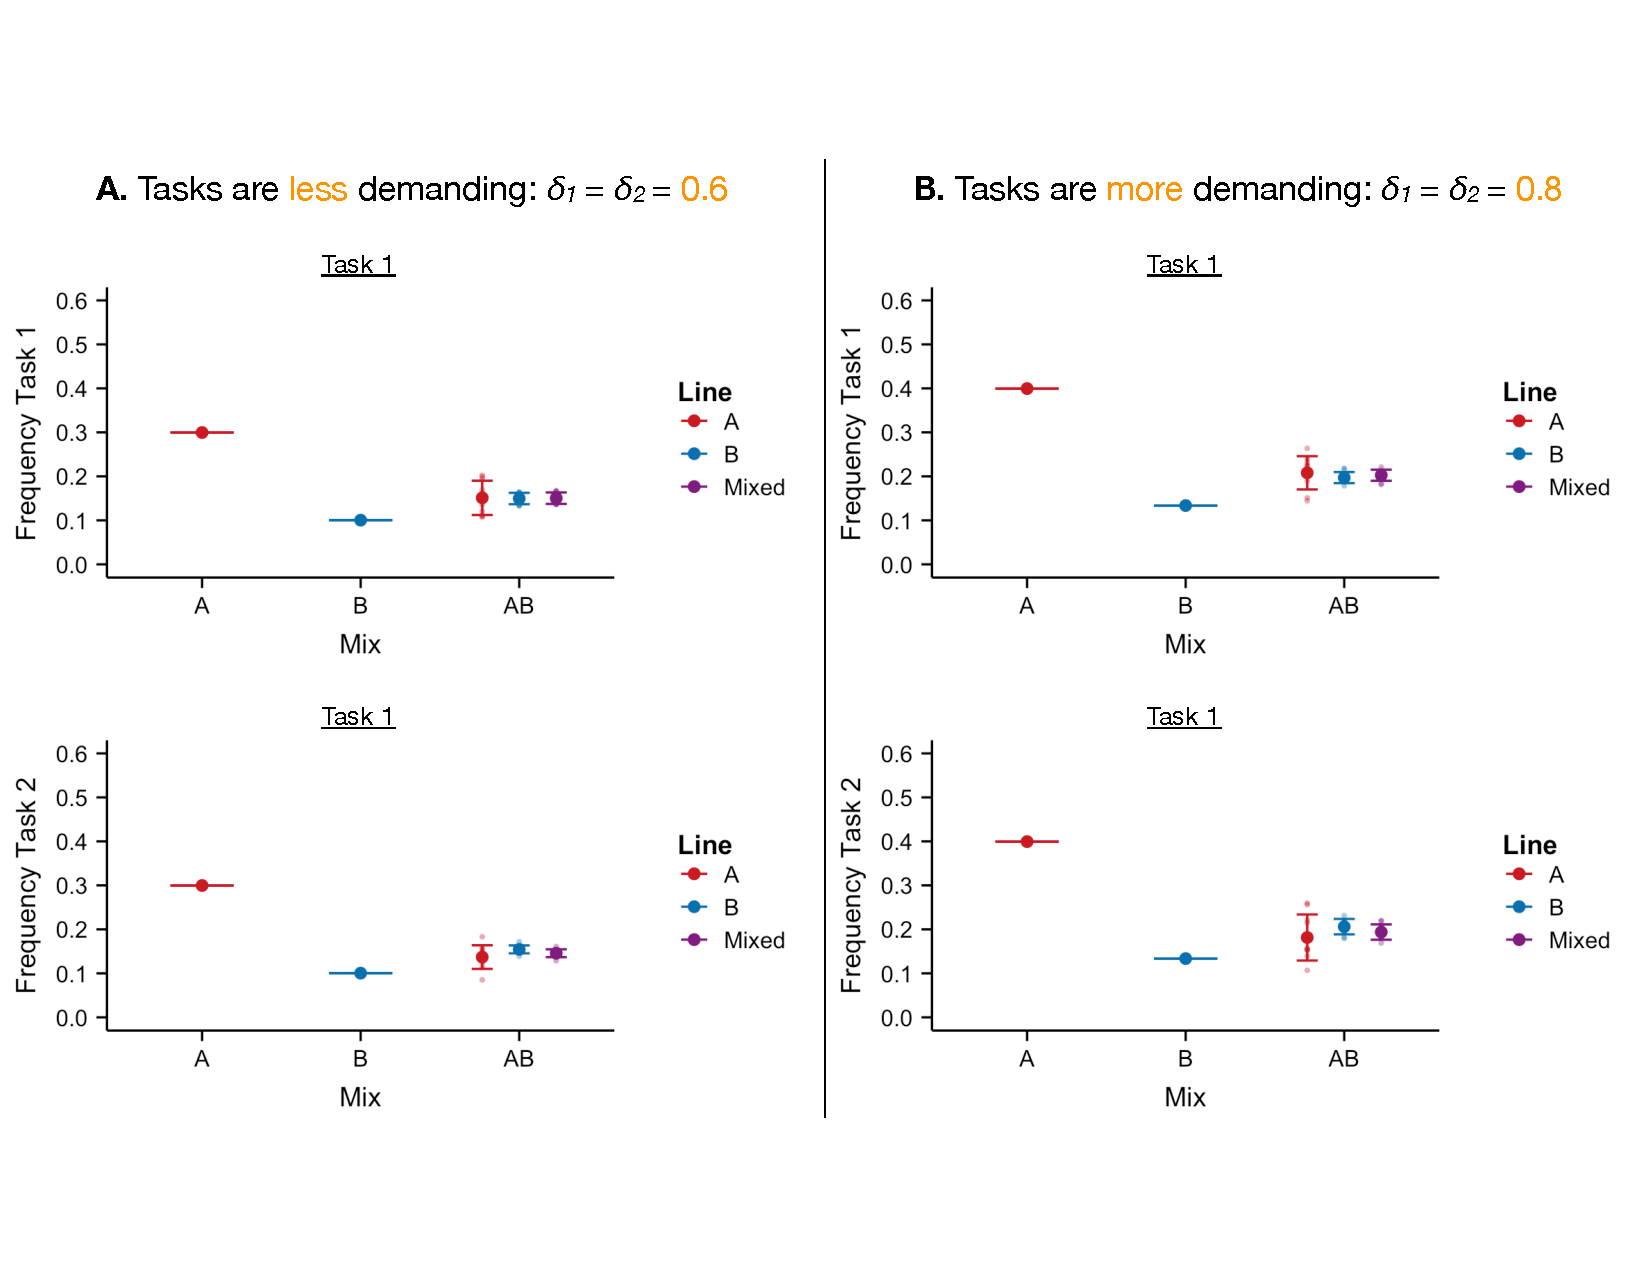
\includegraphics[trim={0 2.75in 0 2.6in}, clip, width=\linewidth]{{doc/deltas_comparison_superefficient}.pdf}
    \caption{Simulation results for varying both the demand rate ($\delta$) and the task efficiency ($\alpha$). For a fixed~$\delta$, line \B\ is more efficient than line \A. \textbf{a}:~Larvae are less demanding ($\delta = 0.6$). \textbf{b}:~Larvae are more demanding ($\delta = 0.8$). Parameters: $\alpha_{j}^{\A} = 2$, $\alpha_{j}^{\B} = 6$, $\sigma = 0.1$, $\mu = 10$, $\eta = 7$.}
    \label{fig:deltassuperefficient}
\end{figure}

% \newpage
Next we explore the scenario where one line is efficient (line \A) and the other is inefficient (line \B); we consider two larval lines (i.e. two values of $\delta$) that maintain this relationship (Fig.~\ref{fig:deltasinefficient}). 
In this case, the ants in the pure-\B\ colonies are more active than those in the pure-\A\ colonies; in the mixed colonies, we observe upward contagions. Changing the demand rate makes no qualitative difference in this relative ordering. 
Note that the task performance level for the inefficient pure-\B\ colonies does not change when $\delta$ changes. This happens because the inefficient \B\ ants---which, by definition (see \hyperref[sec:summary]{Summary}), are unable to meet the colony demands---end up working at maximum capacity in both cases.

% In this case, changing the demand rate changes the picture qualitatively. When larvae are less demanding ($\delta = 0.6$), we observe an upward contagion (Fig.~\ref{fig:deltasinefficient}\textbf{a}); when they are more demanding ($\delta = 0.8$), however, the task performance levels become nearly indistinguishable across the three mixes (Fig.~\ref{fig:deltasinefficient}\textbf{b}). We think that this qualitative change appears because the inefficient ants are unable to keep the stimuli at a steady level: the task performance level for the colony consisting entirely of the inefficient line (pure~\B) remains unchanged for $\delta = 0.6$ and $\delta = 0.8$, which suggests that the ants are working at maximum capacity. When we check the simulation results, we observe that indeed both stimuli keep increasing over time (i.e., do not reach a steady state).

\begin{figure}[H]
    \centering
    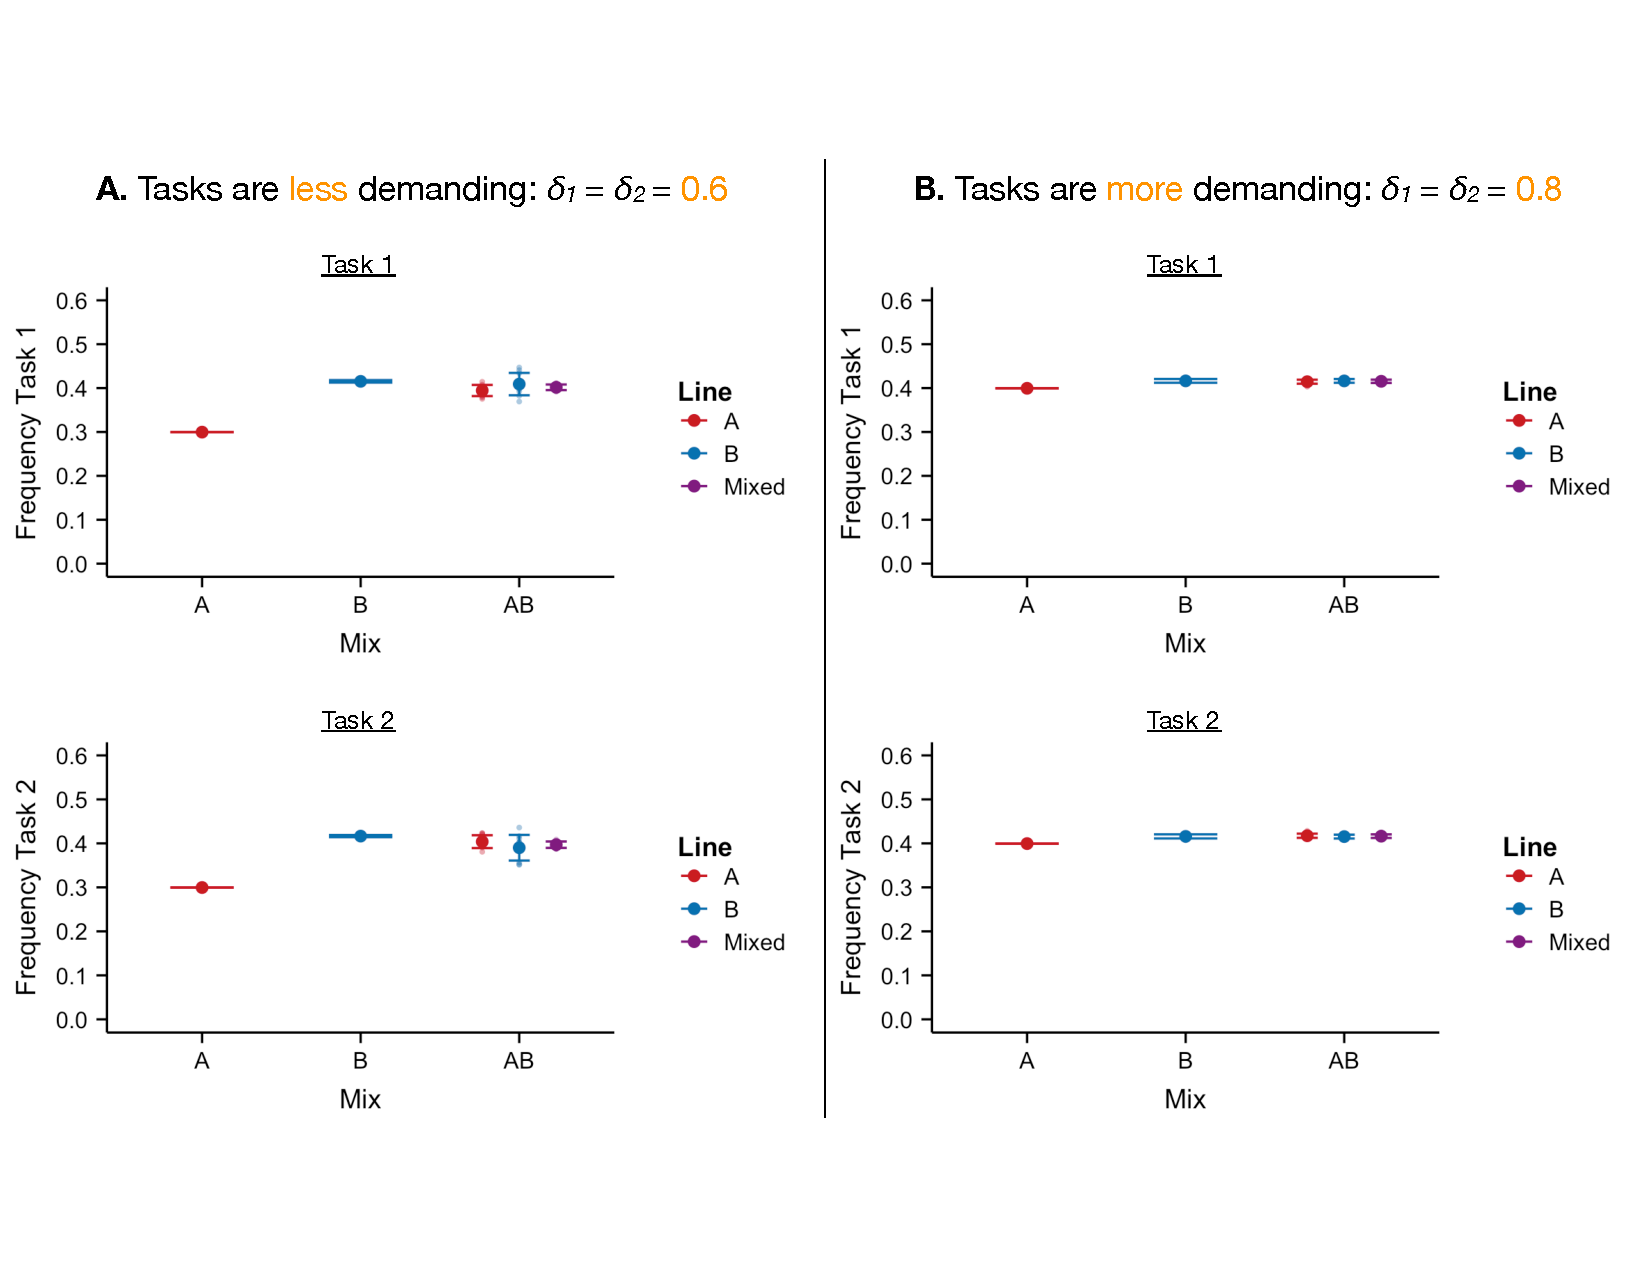
\includegraphics[trim={0 2.75in 0 2.6in}, clip, width=\linewidth]{{doc/deltas_comparison_inefficient}.pdf}
    \caption{Simulation results for varying both the demand rate ($\delta$) and the task efficiency ($\alpha$). For both values of~$\delta$, line \A\ is efficient while line \B\ is inefficient. \textbf{a}:~Larvae are less demanding ($\delta = 0.6$). \textbf{b}:~Larvae are more demanding ($\delta = 0.8$). Parameters: $\alpha_{j}^{\A}  = 2$, $\alpha_{j}^{\B}  = 1$, $\sigma = 0.1$, $\mu = 10$, $\eta = 7$.}
    \label{fig:deltasinefficient}
\end{figure}

% The above observations are based on the case in which one line is more efficient at both tasks than the other line. We also tested the case in which each line is more efficient at one task but less efficient at the other task (e.g., $\alpha_{1}^{\A} = \alpha_{2}^{\B} = 2, \alpha_{1}^{\B} = \alpha_{2}^{\A} = 6$ or $1$). 
% Taken together, the results suggest that \textbf{the demand rate has \textit{no qualitative effect} when all ants are sufficiently efficient but \textit{a nontrivial effect} when some ants are inefficient.}

\newpage
\section{Varying ratios of the genetic lines} \label{sec:varyratios}
Increasing the number of mix ratios demonstrates a non-linear effect with regard to task performance. When exploring these mixes, we held genetic line \A\ as efficient ($\alpha_j^{\A} = 2$) and varied the task efficiency of genetic line \B. The larval type was fixed ($\delta = 0.6$).
When \B\ is more efficient than \A\ ($\alpha_j^{\B} = 6$, Fig.~\ref{fig:Mix_Alphas_B-efficient}), the frequency of task 1 performance increases nonlinearly as the proportion of line \A\ increases. On the other hand, when \B\ is inefficient ($\alpha_j^{\B} = 1$, Fig.~\ref{fig:Mix_Alphas_B-inefficient}), task 1 performance decreases nonlinearly as the proportion of \A\ increases. Overall, this predicts that experiments with more mixing ratios will show a nonlinear trend, assuming that task efficiency is the only difference between the two lines. 

% we held genetic line \A\ as ``average'' in task efficiency (i.e., $\alpha_j^{\A} = 2$) and varied the task efficiency of genetic line \B. For line \B, we assumed either high efficiency (i.e., $\alpha_j^{\B} = 6$) or inefficiency (i.e., $\alpha_j^{\B} = 1$). 
% When \B\ is more efficient than \A\ (Fig.~\ref{fig:Mix_Alphas_B-efficient}), the frequency of task 1 performance increases exponentially as the proportion line \B\ decreases. On the other hand, when \B\ is inefficient (Fig.~\ref{fig:Mix_Alphas_B-inefficient}), task 1 performance decreases non-linearly as the proportion of B increases. Overall, this predicts that experiments with more mixing ratios will show a nonlinear trend, assuming that task efficiency is the main difference between the two lines. 

\begin{figure}[H]
    \centering
    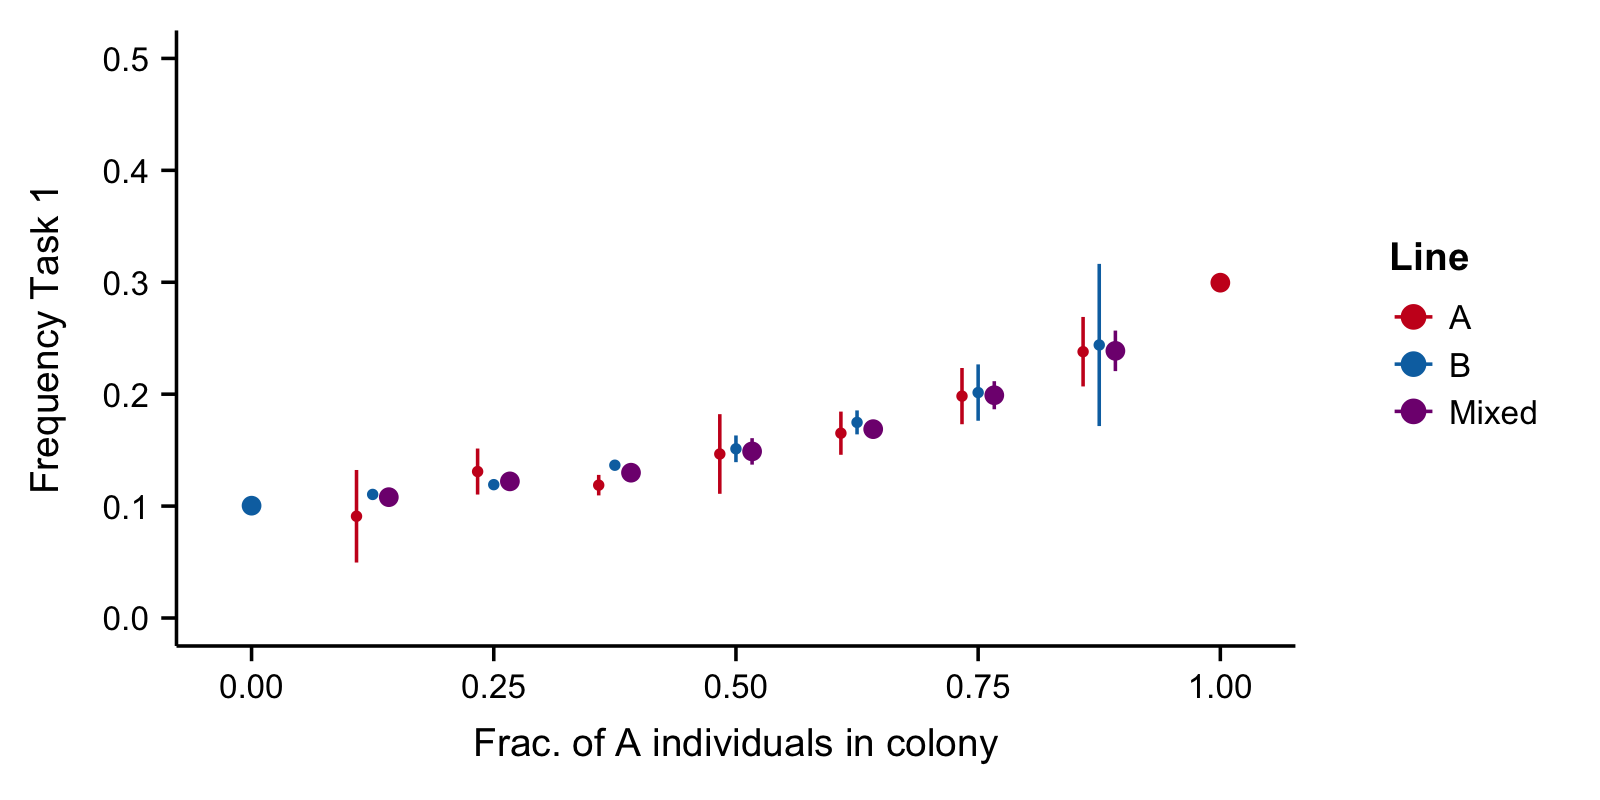
\includegraphics[trim={0 0.25in 0 0.2in}, clip, width=0.9\linewidth]{doc/Mix_Alphas_B-super-efficient_Means.png}
    \caption{Simulation results for mixing of genetic lines when line \B\ is efficient. Parameters: $\alpha_j^{\A}~=~2, \alpha_j^{\B}~=~6.$}
    \label{fig:Mix_Alphas_B-efficient}
\end{figure}

\begin{figure}[H]
    \centering
    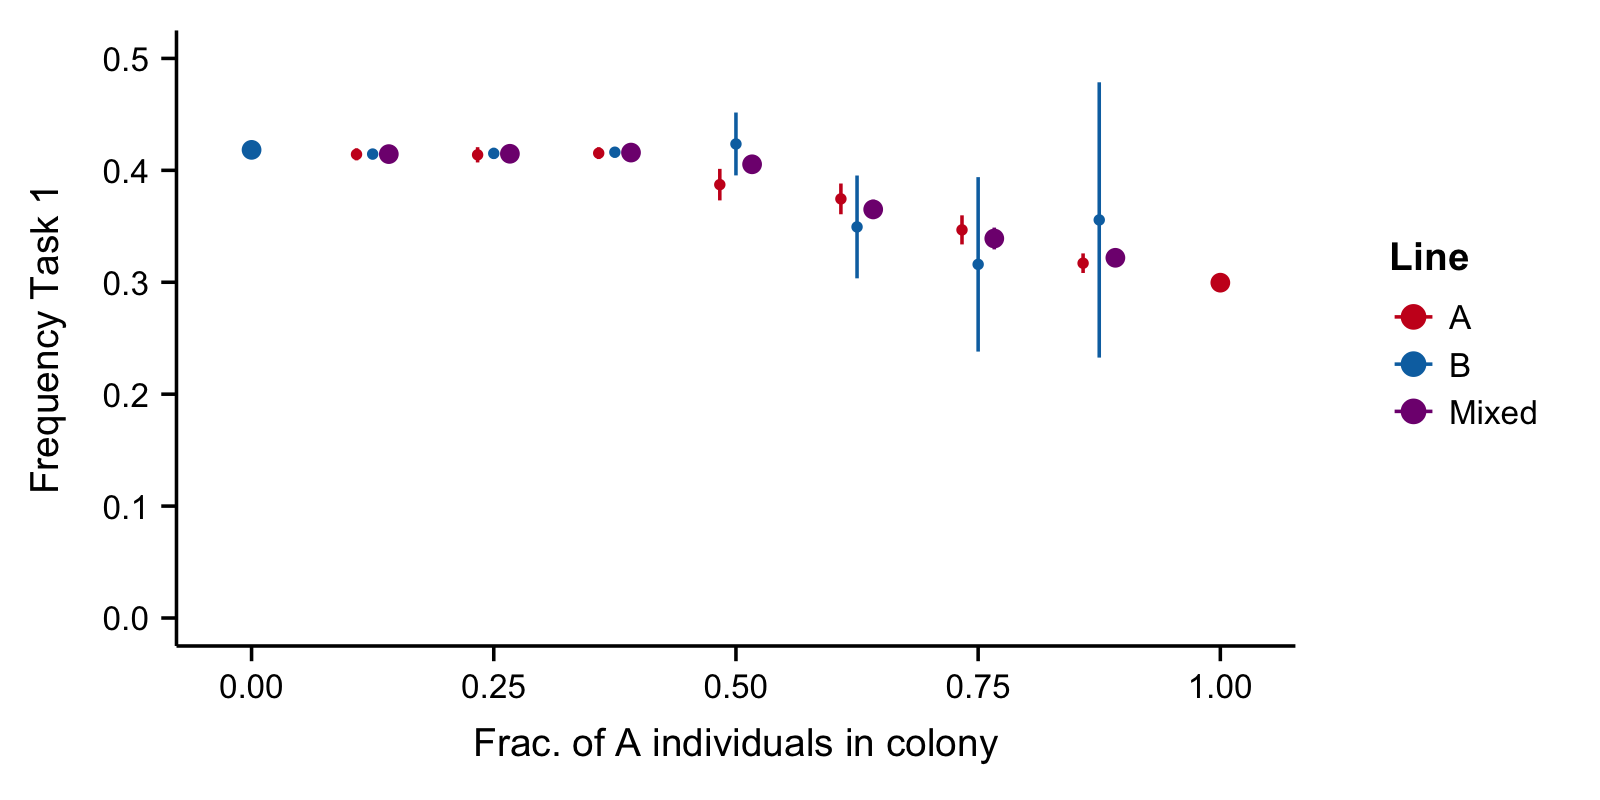
\includegraphics[trim={0 0.25in 0 0.2in}, clip, width=0.9\linewidth]{doc/Mix_Alphas_B-inefficient_Means.png}
    \caption{Simulation results for mixing of genetic lines when line \B\ is inefficient. Parameters: $\alpha_j^{\A}~=~2, \alpha_j^{\B}~=~1.$}
    \label{fig:Mix_Alphas_B-inefficient}
\end{figure}

\section{Varying task efficiency and mean threshold or threshold variance} \label{sec:varyalphamusigma}

\begin{figure}[H]
    \centering
    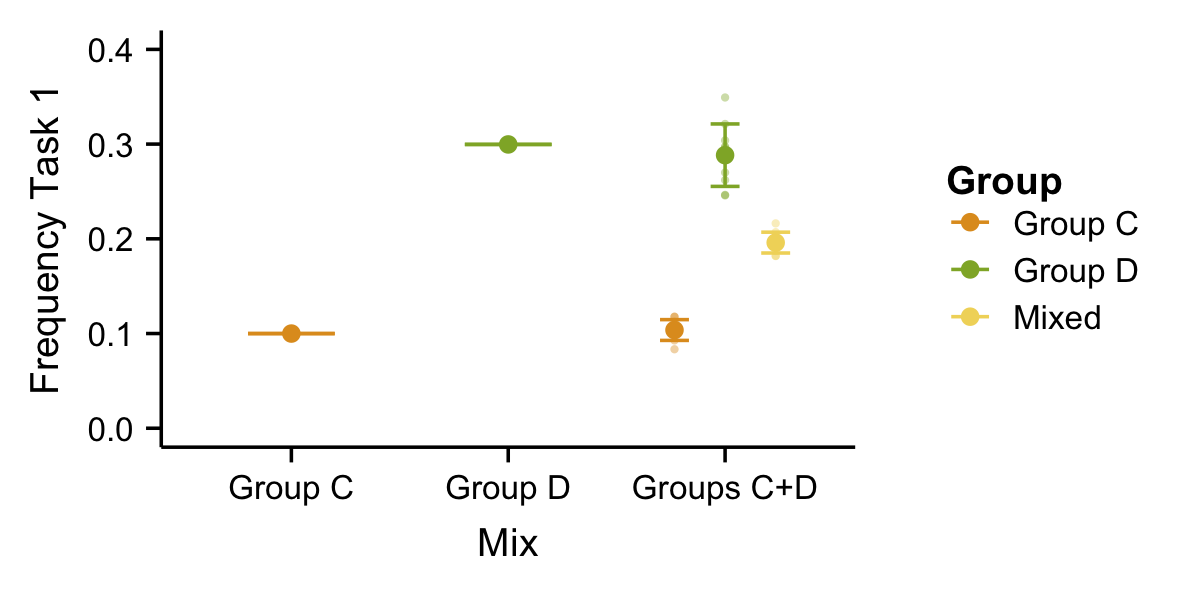
\includegraphics[trim={0 0.25in 0 0.2in}, clip, width=0.9\linewidth]{{doc/AThreshM_14.00_BThreshM_10.00_Task1Morph}.png}
    \caption{Simulation results for the mixing of two groups differing in task efficiency ($\alpha$) and mean threshold ($\mu$). Groups C and D represent demographic (young/old) or morphological {(workers/intercastes)} classes. Parameters: $\alpha_j^{C} = 6, \alpha_j^{D} = 2$, $\mu_j^{C} = 14$, $\mu_j^{D} = 10$.}
    \label{fig:varyalphamu}
\end{figure}

\begin{figure}[H]
    \centering
    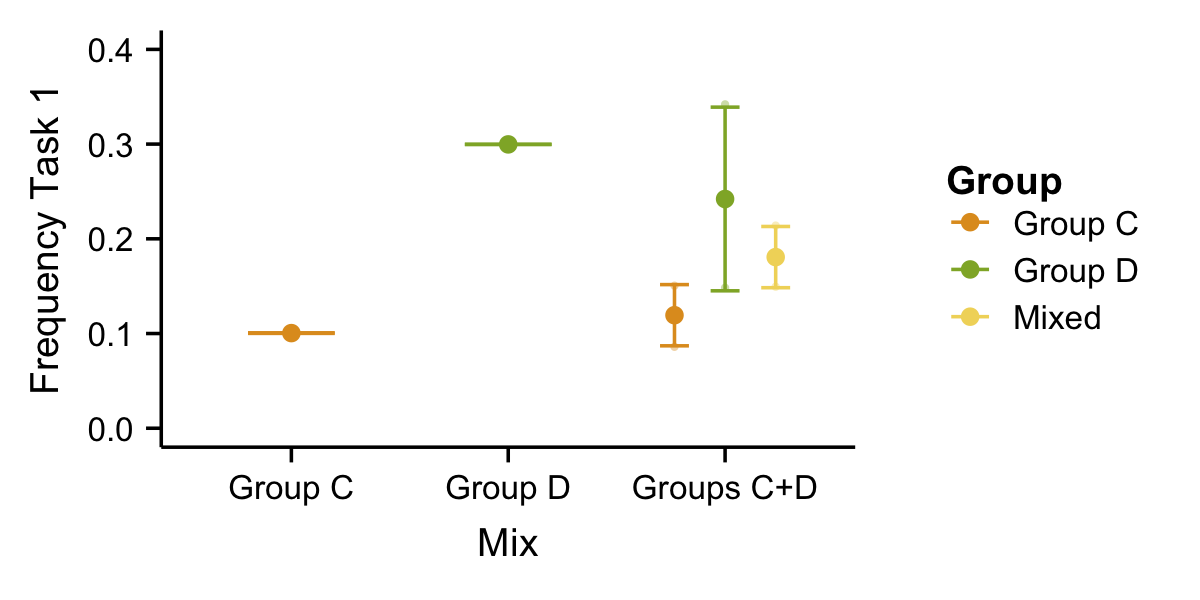
\includegraphics[trim={0 0.25in 0 0.2in}, clip, width=0.9\linewidth]{{doc/AThreshSD_0.10_BThreshSD_0.50_Task1Morph}.png}
    \caption{Simulation results for the mixing of two groups differing in task efficiency ($\alpha$) and threshold variance ($\sigma$). Groups C and D represent demographic (young/old) or morphological {(workers/intercastes)} classes. Parameters: $\alpha_j^{C} = 6, \alpha_j^{D} = 2$, $\sigma_j^{C} = 0.1$, $\sigma_j^{D} = 0.5$.}
    \label{fig:varyalphasigma}
\end{figure}

\newpage
\section{Analytical model} \label{sec:analytical}
% \begin{itemize}
%     \item This is the model
%     \item Here are the predictions that the model makes
%     \item This is what we would like you to test
% \end{itemize}

To better understand our simulation results, we have developed and conducted a preliminary analysis of an analytical model with two different types of ants.  The details of the model and the analysis are outlined in the \hyperref[sec:appendix]{Appendix}; this section summarizes the most important takeaways.

% \textbf{Model summary}.
The model considers $n$ individuals and $m$ tasks. The fractions of line \A\ and \B\ individuals are given by $f$ and $1-f$, respectively. For example, $f=1$ corresponds to a pure \A\ colony, $f = 0.5$ to a 50:50 mixed colony, and $f = 0$ to a pure \B\ colony. 
% As before, $\delta_j$ is the task-specific demand rate, and $\alpha_j^{\A}$ and $\alpha_j^{\B}$ are the task-specific performance efficiencies of lines \A\ and \B, respectively.
The model captures the dynamics of 1) the number of line \A\ and line \B\ individuals performing task $j$ at a given time, denoted $n_{j,t}^{\A}$ and $n_{j,t}^{\B}$ respectively, as well as 2) the stimuli associated with the two tasks. See Appendix~\ref{sec:model} for details.

\subsection{Steady-state predictions 1: varying task efficiency and demand rate} \label{sec:sspred1}
We can analytically predict the task performance level in the steady state when only the task efficiency ($\alpha$) and the demand rate ($\delta$) are varied. Moreover, we can compute the condition under which the system is expected to reach a steady state (See Appendix~\ref{sec:maxactivity} for details). 

Overall, our predictions perform well against the simulations. Figure~\ref{fig:5050_comp} gives two illustrative comparisons. When all the ants in the colony are sufficiently efficient, there is strong agreement between the predicted levels of task performance in the steady state (Fig.~\ref{fig:5050_comp}\textbf{a}). When some ants are inefficient (Fig.~\ref{fig:5050_comp}\textbf{b}), however, colonies violate the necessary condition for reaching a steady state; in this case, our steady-state predictions do not match the simulation results (as we would expect, since the system is not in equilibrium in the first place). A signature of this mismatch is that the stimuli run away (i.e., keep increasing over time).
\begin{figure}[H]
    \centering
    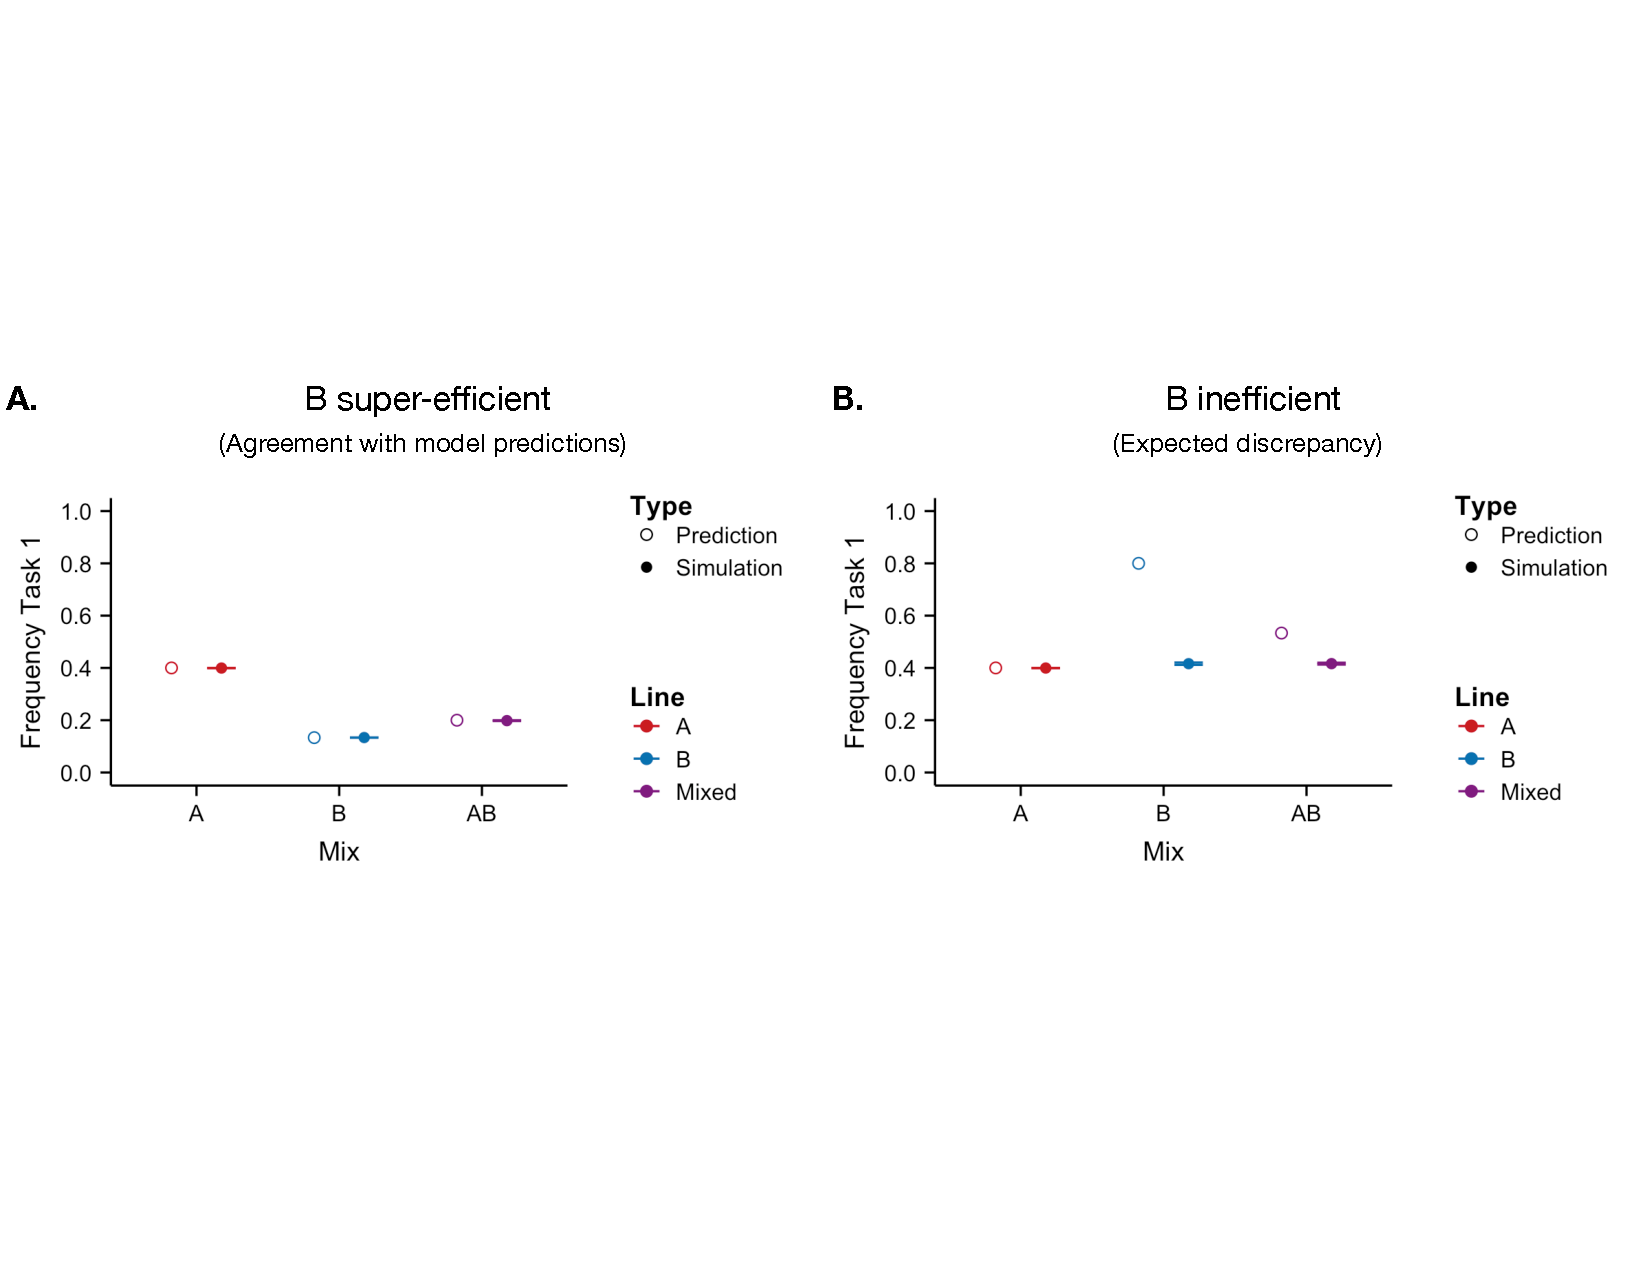
\includegraphics[trim={0 2.5in 0 2.4in}, clip, width=1\linewidth]{doc/model_comparison_deltaalpha.pdf}
    \caption{Comparison of simulation results and analytical predictions of steady states when line \B\ is efficient (\textbf{a}, $\alpha_j^{\B} = 6$) and inefficient (\textbf{b}, $\alpha_j^{\B} = 1$). Line \A\ is efficient in both \textbf{a} and \textbf{b}. Parameters: $\mu = 10, \sigma = 0, \eta = 7, \delta = 0.8$. }
    \label{fig:5050_comp}
\end{figure}

\subsection{Steady-state predictions 2: symmetric mean thresholds} \label{sec:sspred2}
We can also predict the task performance level when the mean thresholds $\mu$ are varied symmetrically ($\mu_{1}^{\A} = \mu_{2}^{\B}$ and $\mu_{2}^{\A} = \mu_{1}^{\B}$) and all other parameters are the same between the two lines and tasks. Figure~\ref{fig:5050_comp_mu} compares two sets of simulation results and predictions. Again, our predictions show strong agreement with the simulation results.
\begin{figure}[H]
    \centering
    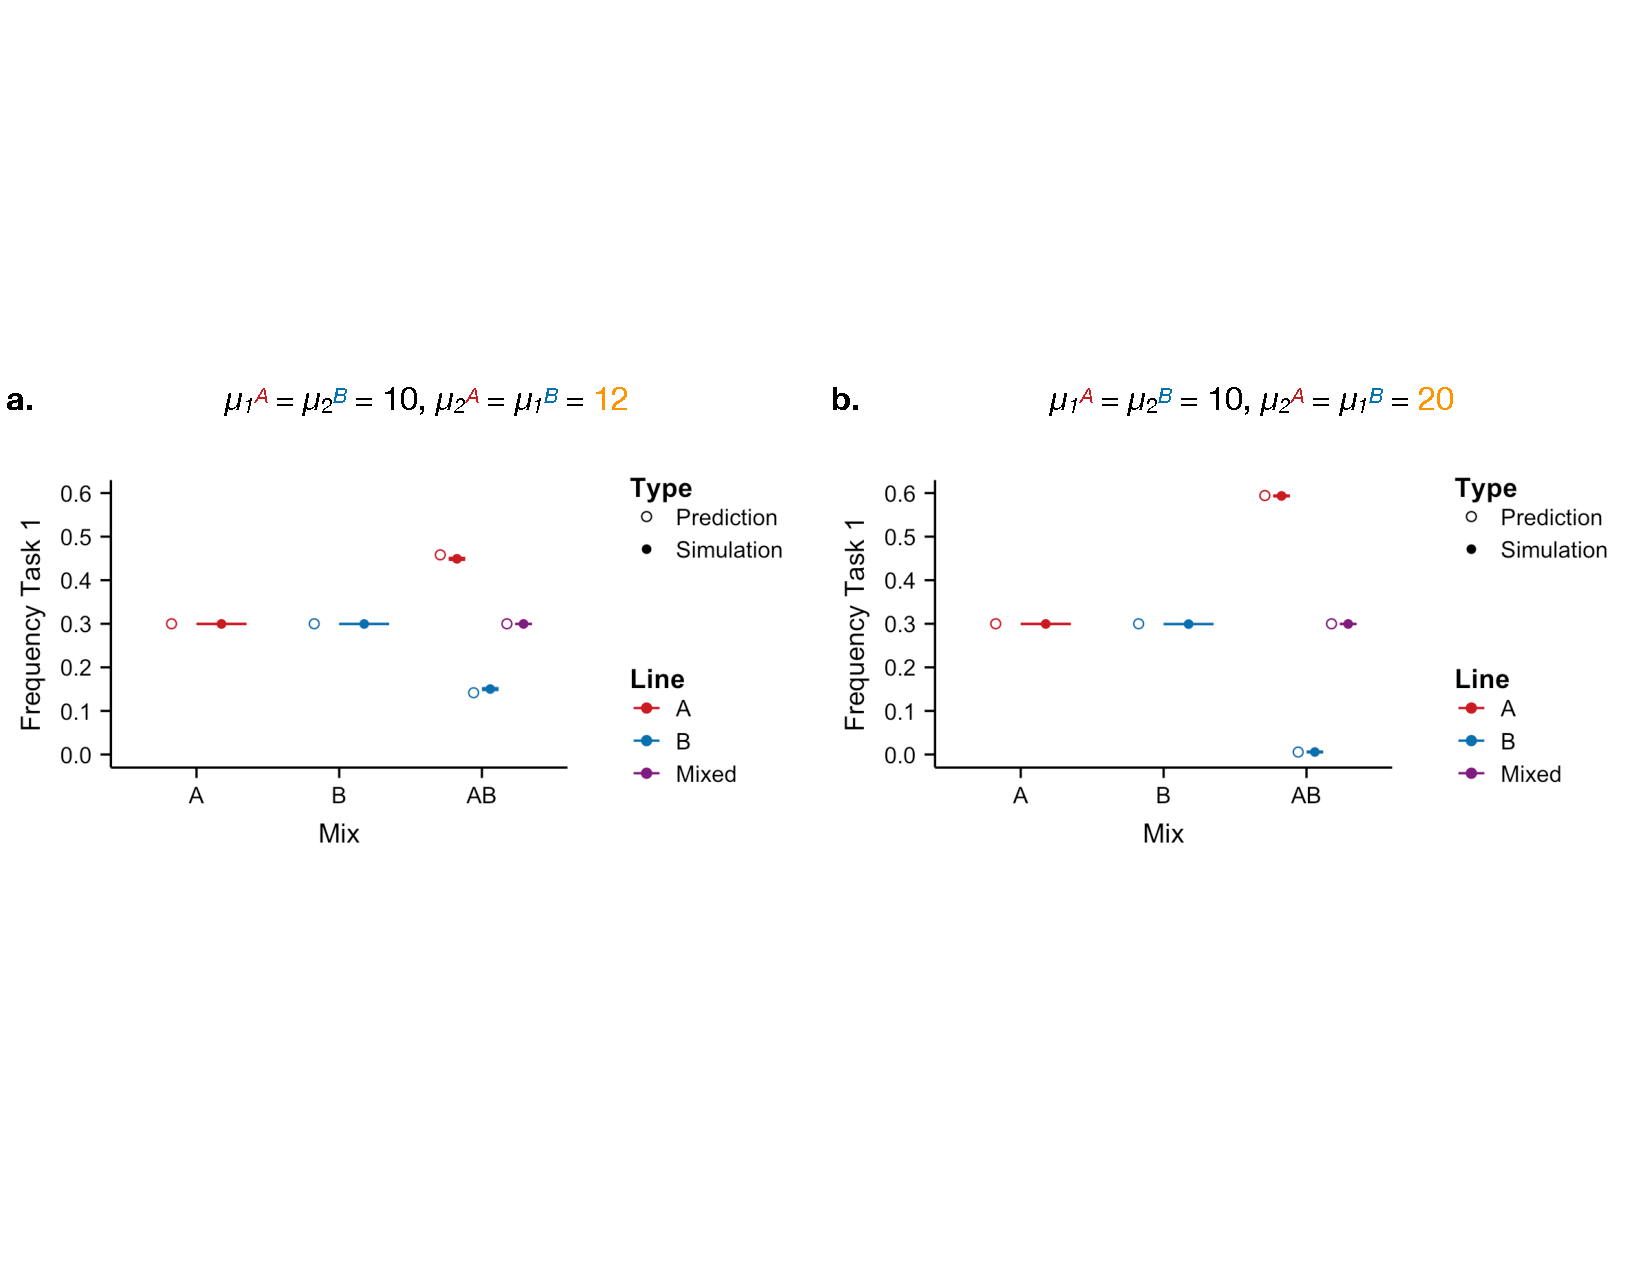
\includegraphics[trim={0 2.6in 0 2.5in}, clip, width=1\linewidth]{doc/model_comparison_mu.pdf}
    \caption{Comparison of simulation results and analytical predictions of steady states
    with symmetric mean thresholds. For both \textbf{a} and \textbf{b}: $\mu_1^{\A} = \mu_2^{\B} = 10$; for \textbf{a}: $\mu_1^{\B} = \mu_2^{\A} = 12$; for \textbf{b}: $\mu_1^{\B} = \mu_2^{\A} = 12$. Other parameters: $\mu = 10, \sigma = 0, \eta = 7, \delta = 0.6, \alpha = 2$. }
    \label{fig:5050_comp_mu}
\end{figure}

% \textbf{Prediction 1}: The ants must be sufficiently efficient in order for the system to reach a steady state (See Section~\ref{sec:maxactivity}). Specifically, the model parameters must satisfy the following condition \later

% \textbf{Prediction 2}: Steady state values

% \textbf{Prediction 3}: Non-50:50 mixes

% \textbf{Prediction 4}: No downward contagion possible for equal $\mu$ and $\tau$.

\subsection{Steady-state predictions 3: varying ratios of genetic lines} \label{sec:sspred3}

As an extension of Section~\ref{sec:sspred1}, we can predict the steady-state task performance level with varied $\delta$ and $\alpha$ across colonies with different genetic ratios.

\begin{figure}[H]
    \centering
    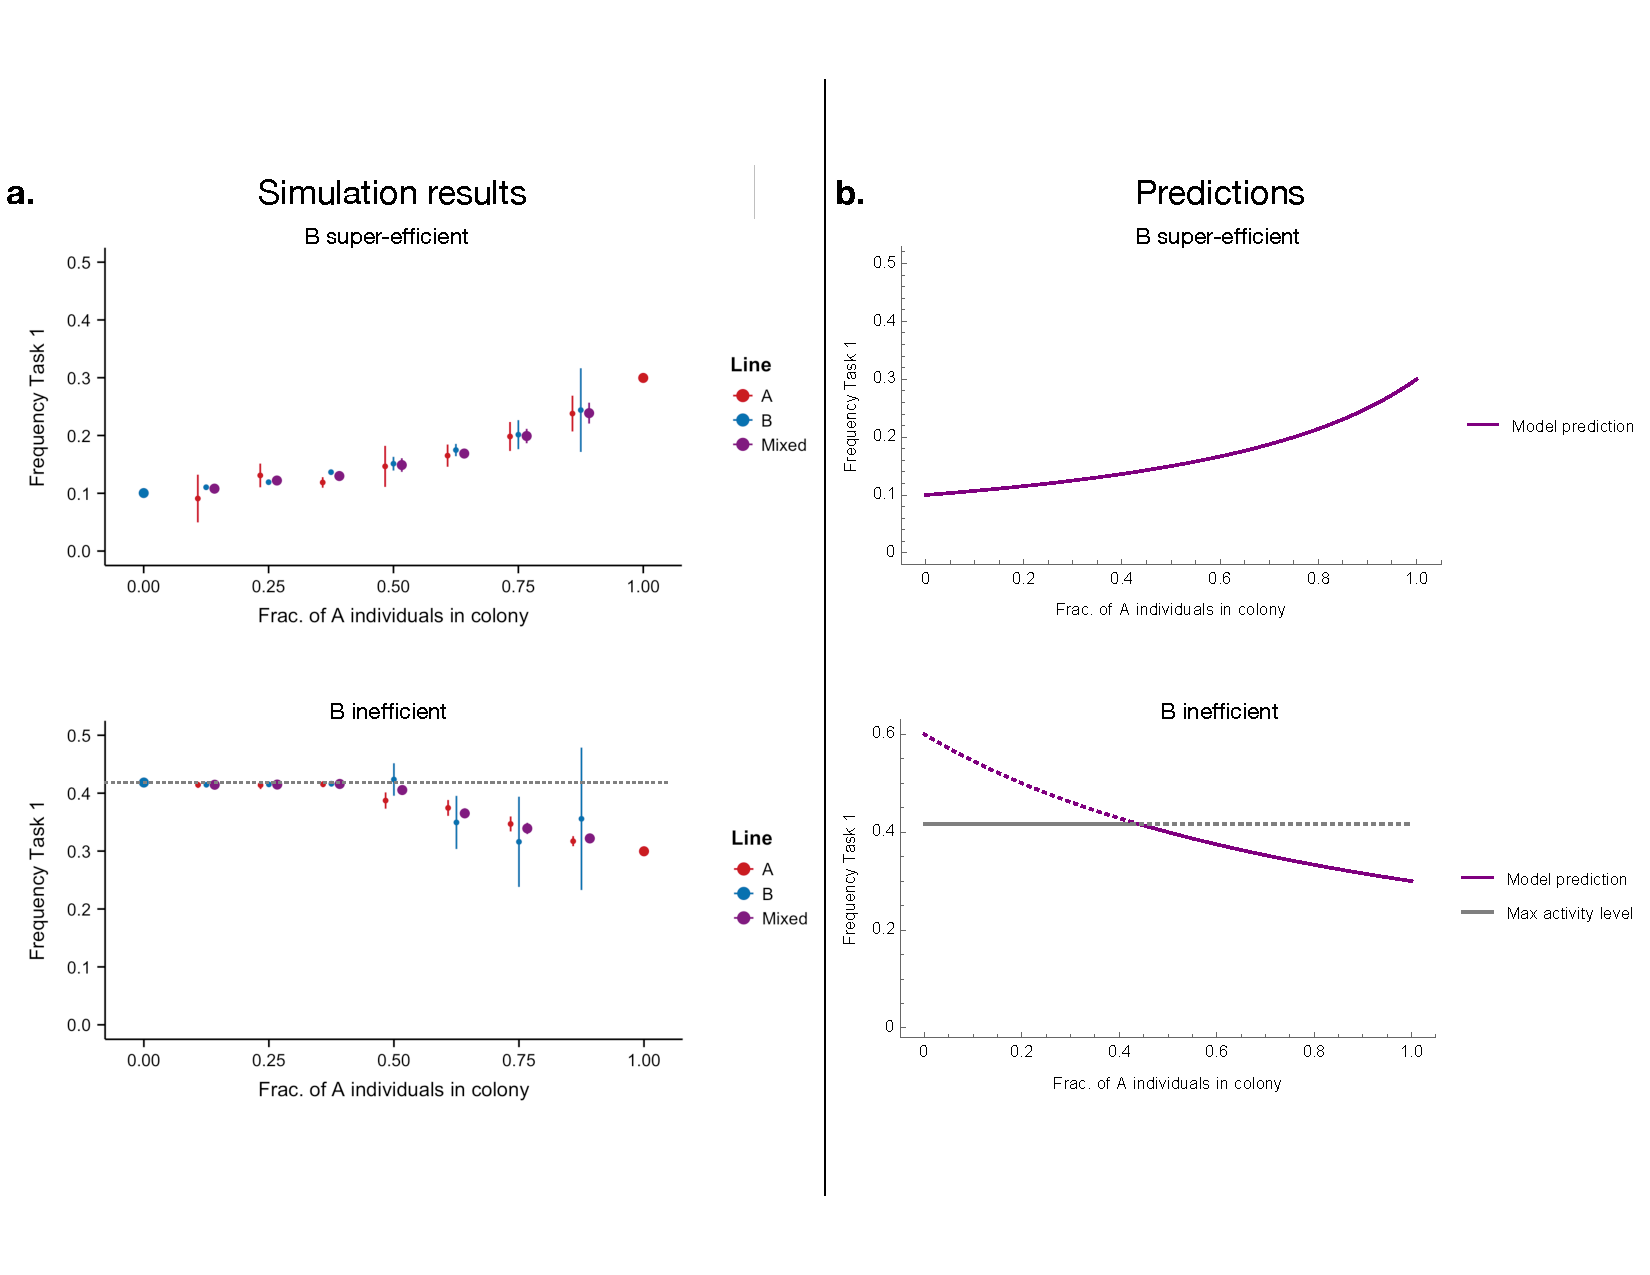
\includegraphics[trim={0 1in 0 1.1in},clip,width=0.95\linewidth]{doc/mixes_comparison.pdf}
    \caption{Comparison of simulation results (\textbf{left}) and analytical predictions (\textbf{right}) with varying ratios of line \A\ and \B\ ants in the colony. \textbf{Top row}: \B\ ants are efficient ($\alpha_j^{\B}=6$). \textbf{Bottom row}: \B\ ants are inefficient ($\alpha_j^{\B}=1$). The gray lines indicate the theoretically predicted maximal activity level for the given parameters (see Appendix~\ref{sec:maxactivity}).
    Parameters: $\mu = 10$, $\delta = 0.6$, $\alpha_j^{\A} = 2$. }
    \label{fig:mixescomp}
\end{figure}

% \subsection{Upward vs. downward contagion} \label{sec:sspred4}

% In our previous discussions, we discussed whether varying both the task efficiency $\alpha$ and the demand rate $\delta$ could capture the difference in the directions of contagion (downward or upward) when the larvae differed. Using the analytical model, we can actually show that, \textit{if the system reaches its steady state, then varying \textbf{only} the demand rate ($\delta$) and task efficiency ($\alpha$) can result in a downward contagion but not an upward contagion} (see Appendix~\ref{sec:updown} for details).

% However, the FTM can still produce an upward contagion if 1) the mean thresholds ($\mu$) are varied in addition to the task efficiencies ($\alpha$) or 2) when at least one of the lines is not sufficiently efficient to maintain the stimuli at constant levels (i.e., reach steady state).

\begin{thebibliography}{99}

\bibitem{ulrich18} Y. Ulrich, J. Saragosti, C. K. Tokita, C. E. Tarnita, D. J. C. Kronauer, ``Fitness benefits and emergent division of labour at the onset of group living,'' \textit{Nature}, vol. 560, pp. 635-638, Aug. 2018.

\bibitem{gautrais02} J. Gautrais, G. Theraulaz, J. L. Deneubourg, C. Anderson, ``Emergent polyethism as a consequence of increased colony size in insect societies,'' \textit{Journal of Theoretical Biology}, vol. 215, pp. 363–373, Apr. 2002.

\end{thebibliography}
\newpage
\begin{appendices}

\section{Analytical model details} \label{sec:appendix}

\subsection{Model} \label{sec:model}

To consider the dynamics of division of labor in mixed colonies, we extend the fixed threshold model in \cite{ulrich18} to incorporate ants of two genetic lines, \A\ and \B. 

The model considers $n$ individuals and $m$ tasks. 
Let $f$ and $1-f$ be the fractions of genetic line \A\ and \B\ individuals in the colony, respectively.
Each task $j$ has an associated stimulus, $s_{j,t}$, at every time $t$, indicating the group-level demand for that task. We model the change in stimulus over discrete time as
\begin{equation}
    s_{j,t+1} - s_{j,t}  = \delta_j - \frac{\alpha_j^{\A} n_{j,t}^{\A} + \alpha_j^{\B} n_{j,t}^{\B} }{n}, \label{eq:stim}
\end{equation}
where $\delta_j$ is the task-specific demand rate; $\alpha_j^{\A}$ and $\alpha_j^{\B}$ are the task-specific performance efficiencies of lines \A\ and \B, respectively; and $n_{j,t}^{\A}$ and $n_{j,t}^{\B}$ are the numbers of line \A\ and line \B\ individuals performing task $j$ and time $t$, respectively.

At each time step, inactive individuals are exposed to the task stimuli randomly until they  either begin performing a task or have encountered all stimuli without landing on a task. Similar to \cite{ulrich18}, our computational model draws individual $i$'s internal threshold $\theta_{ij}$ for task $j$ from a normal distribution with mean $\mu_j$ and normalized standard deviation $\sigma_j$ (each of which can be line- and/or task-specific). To gain analytical insight into the model, we make the simplifying assumption that $\sigma_j = 0$ for all tasks.
In other words, \textit{we assume that the line- and task-specific thresholds are given by the constant parameters, $\mu_j^{\A}$ and $\mu_j^{\B}$.}
With this assumption, the probabilities $P_{ij,t}^{\A}$ and $P_{ij,t}^{\B}$ that inactive individuals $i$ of lines \A\ and \B\ begin to perform task $j$ at time $t$ can be written respectively as
\begin{equation}
    P_{j,t}^{\A} (s_{j,t}) = \frac{s_{j,t}^\eta}{s_{j,t}^\eta + {(\mu_j^{\A})}^\eta}, \quad P_{j,t}^{\B} (s_{j,t}) = \frac{s_{j,t}^\eta}{s_{j,t}^\eta +{(\mu_j^{\B})}^\eta}.
\end{equation}
The parameter $\eta$ governs the steepness of the response threshold function as in the original model.

Finally, at time $t$, active individuals quit their tasks with a constant quit probability $\tau$. In the case of two tasks ($m = 2$), the numbers of line \A\ and line \B\ individuals working on task $j$ change according to the following:
\begin{align}
    n_{j,t+1}^{\A} - n_{j,t}^{\A}  & =  \frac{1}{2} \bigg[ P_{j,t}^{\A}(s_{j,t}) + (1 - P_{j',t}^{\A}(s_{j',t}))P_{j,t}^{\A}(s_{j,t})\bigg] \bigg( fn
 - (n_{j,t}^{\A} + n_{j',t}^{\A}) \bigg) - \tau n_{j,t}^{\A} \nonumber\\
    n_{j,t+1}^{\B} - n_{j,t}^{\B}  & = \frac{1}{2} \bigg[ P_{j,t}^{\B}(s_{j,t}) + (1 - P_{j',t}^{\B}(s_{j',t}))P_{j,t}^{\B}(s_{j,t})\bigg] \bigg( (1-f)n - (n_{j,t}^{\B} + n_{j',t}^{\B}) \bigg) - \tau n_{j,t}^{\B} \label{eq:active}
\end{align}
for $(j,j')=(1,2), (2,1)$. {\color{black}The sums in square brackets capture the possible ways in which individuals can initiate task $j$: they can either encounter the stimulus for task $j$ immediately and begin performing that task, or they can first encounter the stimulus for the other task $j'$, decide not to perform that task, subsequently encounter the stimulus for task $j$, and begin performing task $j$.}

The full model with two tasks ($m=2$) consists of the six equations describing changes in $s_1, s_2$~\eqref{eq:stim} and $ n_1^{\A}, n_1^{\B}, n_2^{\A}, n_2^{\B}$~\eqref{eq:active}. 
% Exclude for now
% Given initial conditions 
% % $s_{1,0} \geq 0$, $s_{2,0} \geq 0$, 
% $0\leq n_{1,0}^{\A}+n_{2,0}^{\A} \leq fn$ and $0\leq n_{1,0}^{\B}+ n_{2,0}^{\B} \leq (1-f)n$,
% the dynamics will satisfy the constraints $0\leq n_{1,t}^{\A}+n_{2,t}^{\A} \leq fn$ and $0\leq n_{1,t}^{\B}+ n_{2,t}^{\B} \leq (1-f)n$ for all $t \geqq 0$.

\subsection{Steady-state predictions}
To understand how well the analtyical model captures the simulation results, we investigate the steady-state predictions of the analytical model for two tasks ($m=2$).

\subsubsection{A necessary condition for the existence of a biologically plausible equilibrium} \label{sec:maxactivity}

In our computational model, the individuals essentially have a latency period of one time step between when they quit a task and recommence working. This means that, on average, only a fraction of the colony can be working at any given time.

To find this maximal activity level, let $X_t = (n_{1,t}^{\A}+ n_{1,t}^{\B}+ n_{2,t}^{\A}+n_{2,t}^{\B})/n$ be the fraction of active individuals in a colony at time $t$. Note that $0\leq X_t\leq 1$. At time $t+1$, a fraction $\tau X_t$ of the colony is expected to be inactive. Therefore, at time $t+1$,
\begin{equation}
    \mathrm{(fraction\ active)} + \mathrm{(fraction\ inactive)}  = X_{t+1} + \tau X_t \leq 1.
\end{equation}
At steady state, $X_{t+1} = X_{t} = X^*$. By substitution, we obtain a necessary condition for a biologically plausible steady state to exist:
\begin{equation}
    X^* \leq \frac{1}{1+\tau}. \label{eq:maxactivity}
\end{equation}
For example, for $\tau = 0.2$ used in the simulations below, at most $83.33$\% of the individuals in a colony can be active at steady state.
A similar condition for the theoretically possible maximum activity level at steady state has been noted in \cite{gautrais02}.

\subsubsection{Pure colonies: 2 tasks, 1 line} \label{sec:pure}
For pure (\A-only) colonies, we set $f = 1$ and $n_{j,t}^{\B} = 0$ for all time $t$. Setting Eq.~\eqref{eq:stim} to zero, we obtain
\begin{equation}
    \frac{n_j^{\A}}{n} = \frac{\delta_j}{\alpha_j^{\A}}
    \label{eq:ss1}
\end{equation}
as the fraction of \A\ ants performing task $j$ at steady state.

Notably, the steady-state values of $n_j^{\A}$ are \textit{independent} of the mean threshold ($\mu_j^{\A}$) or the quit probability ($\tau^{\A}$). This agrees with the results of our simulations, where varying $\mu$ and $\tau$ by line did not lead to differing mean task performance levels in the pure colonies.

According to condition \eqref{eq:maxactivity}, this steady state is biologically possible only if
\begin{equation}
    (X^* =)\ \frac{n_1^{\A}}{n} + \frac{n_2^{\A}}{n} = \frac{\delta_1}{\alpha_1^{\A}} + \frac{\delta_2}{\alpha_2^{\A} }\leq \frac{1}{1+\tau} \label{eq:cond1}.
\end{equation}
If this condition is not met, then we would expect the stimuli to continue growing (i.e., the system will not reach a steady state).


\subsubsection{Mixed colonies: 2 tasks, 2 lines, 50:50 mixes} \label{sec:5050}

We now consider the 50:50 mixes ($f=0.5$), i.e., mixed colonies consisting of an equal number of \A\ and \B\ ants.
Here we assume that the mean thresholds and the quit probabilities are identical for both tasks and lines ($\mu_1^{\A} = \mu_2^{\A} = \mu_1^{\B} = \mu_2^{\B}$ and $\tau^{\A} = \tau^{\B}$)\footnote{The parameters $\mu$ and $\tau$ do not explicitly appear in \eqref{eq:ss2} when we assume that the mean thresholds are identical for all individuals and both tasks. However, based on the Eqs.~\eqref{eq:active}, we expect the general form of steady state fractions of active individuals to be explicit functions of $\mu_j^{\A}$ and $\mu_j^{\B}$ as well as $\tau^{\A}$ and $\tau^{\B}$. The steady states can be computed numerically for the case when these parameters vary, but the analytical expression is too complicated to write down.}, as we have done in the simulations with varied $\delta$ and $\alpha$ values. Setting Eqs.~\eqref{eq:stim} and \eqref{eq:active} equal to zero, we find the steady-state numbers of individuals performing task $j$ as
\begin{equation}
     n_j^{\A} =  n_j^{\B} = n\bigg(\frac{\delta_j}{\alpha_j^{\A} + \alpha_j^{\B}}\bigg). \label{eq:ss2a}
\end{equation}
Alternatively, as fractions of each genetic type of individuals,
\begin{equation}
     \frac{n_j^{\A}}{(n/2)} =  \frac{n_j^{\B}}{(n/2)} = \frac{2\delta_j}{\alpha_j^{\A} + \alpha_j^{\B}}. \label{eq:ss2}
\end{equation}
Applying condition \eqref{eq:maxactivity}, this state state exists only if
\begin{equation}
     (X^*=)\ \sum_{j=1}^2 \frac{n_j^{\A}}{n} + \frac{n_j^{\B}}{n} 
     = \sum_{j=1}^2 \frac{2\delta_j}{\alpha_j^{\A} + \alpha_j^{\B}}
     \leq \frac{1}{1+\tau}.
     \label{eq:cond2}
\end{equation}
Again, if this condition is not met, then we would expect the stimuli to continue growing over time and for the ants to be working at max capacity.

\subsubsection{Mixed colonies: 2 tasks, 2 lines, non-50:50 mixes}

We now generalize to the case in which a fraction $f$ of individuals in a mixed colony are of genetic line \A. In the simplified case where $\mu_1^{\A} = \mu_2^{\A} = \mu_1^{\B} = \mu_2^{\B}$ and $\tau^{\A} = \tau^{\B}$, the steady-state fractions of individuals performing task $j$ are
\begin{equation}
     n_j^{\A} =  \frac{fn\delta_j}{f\alpha_j^{\A} + (1-f)\alpha_j^{\B}}, 
     \quad
     n_j^{\B} =  \frac{(1-f)n\delta_j}{f\alpha_j^{\A} + (1-f)\alpha_j^{\B}}, 
     \label{eq:ss3a}
\end{equation}
or, as fractions of the individuals of each genetic type (recall that there are $fn$ individuals of type \A\ and $(1-f)n$ individuals of type \B),
\begin{equation}
     \frac{n_j^{\A}}{fn} =  \frac{n_j^{\B}}{(1-f)n} = \frac{\delta_j}{f\alpha_j^{\A} + (1-f)\alpha_j^{\B}} \ \bigg(= \frac{n_j^{\A} + n_j^{\B}}{n}\bigg). \label{eq:ss3}
\end{equation}
The last equality highlights the fact that the fraction of individuals \textit{of each type} performing task $j$ is identical to the fraction \textit{of the whole colony} performing that task. As expected, the expressions \eqref{eq:ss3} reduce to \eqref{eq:ss2} when $f=0.5$ (50:50 mixes) and to \eqref{eq:ss1} when $f=1$ (pure \A\ colonies). Again, we would expect to see this equilibrium only when condition \eqref{eq:maxactivity} is satisfied. 

From these results, we would expect the steady-state fraction of task $j$ performance frequency (which corresponds to \eqref{eq:ss3}) to depend \textit{nonlinearly} on the fraction of \A\ individuals ($f$). 
\subsubsection{Mixed colonies: 2 tasks, 2 lines, 50:50 mixes, symmetric mean thresholds}

So far we have assumed that the mean thresholds $\mu_{j}^{\A}$ and $\mu_{j}^{\B}$ were identically for both lines and tasks ($\mu_{1}^{\A} = \mu_{2}^{\A} = \mu_{1}^{\B} = \mu_{2}^{\B}$). While the system of equations can be solved numerically even when we vary $\mu$, the steady-state expressions quickly become too complicated to write down.

In the following special case, however, we can express the equilibrium values exactly. Assume that 
\begin{itemize}
    \item 1) the task efficiencies are the same for both lines and tasks ($\alpha_{1}^{\A} = \alpha_{2}^{\A} = \alpha_{1}^{\B} = \alpha_{2}^{\B} = \alpha$);
    \item 2) the quit probabilities are the same for both tasks ($\tau^{\A} = \tau^{\B} = \tau$); and
    \item 3) the task demand rates are the same for both tasks ($\delta_1 = \delta_2  = \delta$); 4) the task thresholds are ``symmetric'': $\mu_{1}^{\A} = \mu_{2}^{\B} = a$ and $\mu_{2}^{\A} = \mu_{1}^{\B} = b$. 
\end{itemize}

The symmetry of the parameters means that the dynamics of the stimuli are identical. Therefore, at steady state, the stimulus levels should be equal ($s_1 = s_2 = s$). Moreover, the number of \A\ ants performing task 1 should be identical to that of \B\ ants performing task 2 ($n_{1}^{\A} = n_{2}^{\B}$) and the number of \B\ ants performing task 1 should be identical to that of \A\ ants performing task 2 ($n_{1}^{\B} = n_{2}^{\A}$).

Taking advantage of this symmetry, we can write down the steady-state stimulus level $s$ $(=s_1 = s_2)$ as
\begin{equation}
    s^* = \bigg[\frac{1}{2} \bigg( -({a}^\eta + {b}^\eta) 
    \pm \sqrt{
    ({a}^\eta + {b}^\eta)^2 + ({a}^\eta {b}^\eta)\cdot \frac{8\delta \tau}{\alpha - 2\delta (1+\tau)}
    } \bigg)\bigg]^\frac{1}{\eta}.
\end{equation}
The corresponding steady-state fractions of \A\ and \B\ ants performing tasks 1 and 2 are
\begin{equation}
    \frac{n_1^{\A}}{(n/2)} =  \frac{n_2^{\B}}{(n/2)} = \frac{1}{\tau} \bigg(\frac{(s^*)^\eta}{(s^*)^\eta + {a}^\eta} \bigg)\bigg[2 - \frac{(s^*)^\eta}{(s^*)^\eta + {b}^\eta}  \bigg] \bigg(\frac{1}{2} - \frac{\delta}{\alpha} \bigg)
    \label{eq:sol4}
\end{equation}
\begin{equation}
    \frac{n_2^{\A}}{(n/2)} =  \frac{n_1^{\B}}{(n/2)}  = \frac{1}{\tau} \bigg(\frac{(s^*)^\eta}{(s^*)^\eta + {b}^\eta} \bigg)\bigg[2 - \frac{(s^*)^\eta}{(s^*)^\eta + {a}^\eta}  \bigg] \bigg(\frac{1}{2} - \frac{\delta}{\alpha} \bigg)
    \label{eq:sol5}
\end{equation}
When $a = b$ (i.e., when all $\mu$'s are the same), \eqref{eq:sol4} and \eqref{eq:sol5} reduce to the steady-state values predicted in \eqref{eq:ss2}.

\subsection{Downward vs. upward contagion} \label{sec:updown}

One question that was raised during our previous discussion was whether varying both the task efficiency $\alpha$ and the demand rate $\delta$ would capture the difference in the directions of contagion (downward or upward) when the larvae differed. In Section~\ref{sec:varyalphadelta}, we presented simulation results that suggest that upward contagion only occurs when some of the ants are inefficient and therefore the colony cannot maintain the stimuli at a steady level. Here we show analytically that, \textit{if the system reaches its steady state (i.e., condition \eqref{eq:maxactivity} is satisfied), then varying \textbf{only} the demand rate ($\delta$) and task efficiency ($\alpha$) can result in a downward contagion but not an upward contagion.}

If we only vary $\delta$ and $\alpha$, then the mean thresholds and the quit probabilities are identical across tasks and lines. So we can directly apply the steady-state fractions of active individuals computed in Eqs.~\eqref{eq:ss1} and \eqref{eq:ss2}. The behavioral contagion is ``downward'' if
\begin{equation}
    \frac{1}{2} \bigg( \frac{\delta_j}{\alpha_j^{\A}} + \frac{\delta_j}{\alpha_j^{\B}} \bigg) > \frac{2\delta_j}{\alpha_j^{\A} + \alpha_j^{\B}} \label{eq:down}
\end{equation}
and ``upward'' if the inequality is reversed (the schematic in Fig.~\ref{fig:schematic} should help).
\begin{figure}[H]
    \centering
    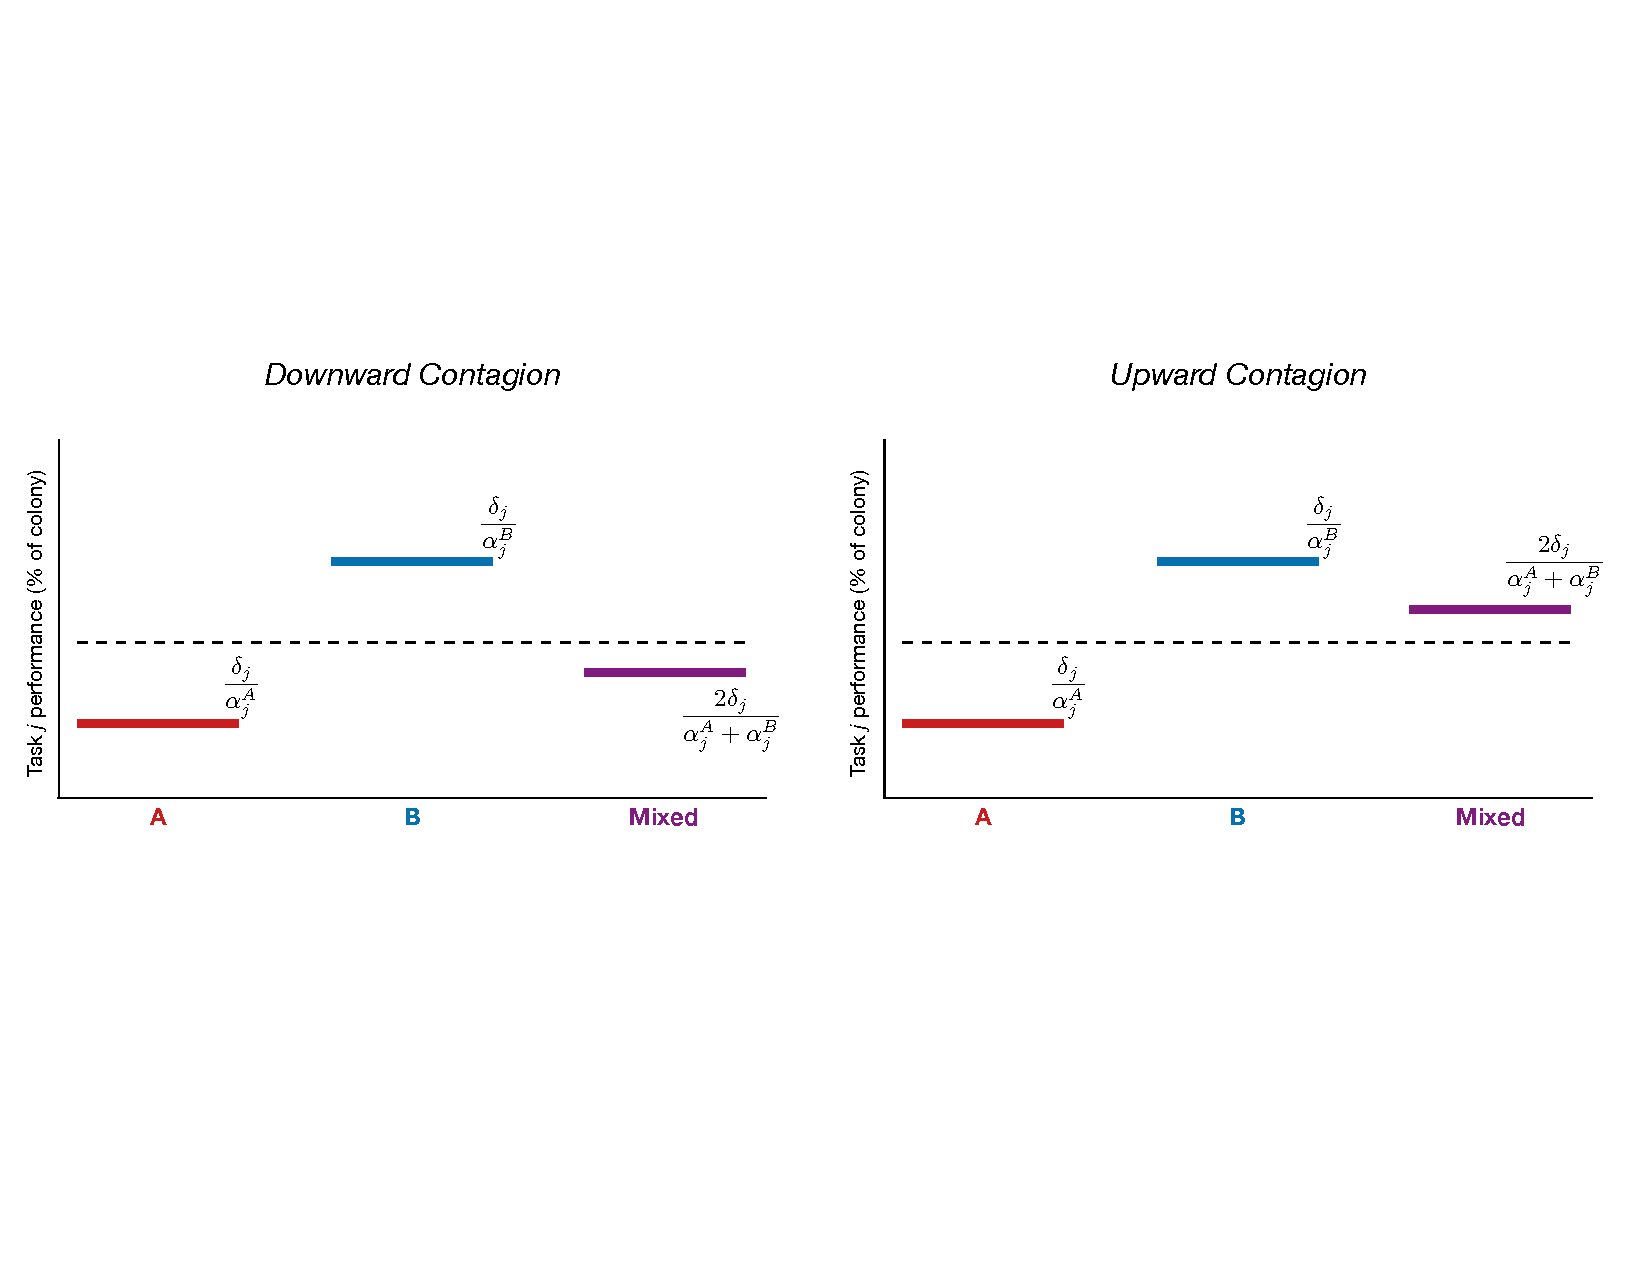
\includegraphics[width=0.9\linewidth]{doc/schematic_contagion.pdf}
    \caption{A schematic representing the two contagion patterns of our interest. The task $j$ performance (\%) values for the mixed colonies assume that the mean thresholds and the quit probabilities are identical for both lines and both tasks ($\mu_1^{\A} = \mu_2^{\A} = \mu_1^{\B} = \mu_2^{\B}$ and $\tau^{\A} = \tau^{\B}$).}
    \label{fig:schematic}
\end{figure}
\noindent By manipulating the inequality \eqref{eq:down}, however, we see that the LHS is always at least as large as the RHS:
\begin{align}
    \frac{1}{2} \bigg( \frac{\delta_j}{\alpha_j^{\A}} + \frac{\delta_j}{\alpha_j^{\B}} \bigg) - \frac{2\delta_j}{\alpha_j^{\A} + \alpha_j^{\B}} 
    % & = \frac{\delta_j}{2} \bigg( \frac{1}{\alpha_j^{\A}} + \frac{1}{\alpha_j^{\B}} - \frac{4}{\alpha_j^{\A} + \alpha_j^{\B}} \bigg) \nonumber\\
    % & = \frac{\delta_j}{2} \Bigg( 
    % \frac{\alpha_j^{\B} (\alpha_j^{\A} + \alpha_j^{\B}) + \alpha_j^{\A} (\alpha_j^{\A} + \alpha_j^{\B}) - 4\alpha_j^{\A}\alpha_j^{\B}}{\alpha_j^{\A}\alpha_j^{\B}(\alpha_j^{\A} + \alpha_j^{\B})} \Bigg) \nonumber\\
    % & = \frac{\delta_j}{2} \Bigg( 
    % \frac{ (\alpha_j^{\A})^2 + (\alpha_j^{\B})^2 - 2\alpha_j^{\A}\alpha_j^{\B}}{\alpha_j^{\A}\alpha_j^{\B}(\alpha_j^{\A} + \alpha_j^{\B})} \Bigg) \nonumber\\
    & = \frac{\delta_j}{2} \Bigg( 
    \frac{ (\alpha_j^{\A} - \alpha_j^{\B})^2 }{\alpha_j^{\A}\alpha_j^{\B}(\alpha_j^{\A} + \alpha_j^{\B})} \Bigg) \geq 0
\end{align}
The equality holds if and only if $\alpha_j^{\A} = \alpha_j^{\B}$, in which case the ants are indistinguishable with respect to task~$j$ (the three lines take the same value for task $j$). If $\alpha_j^{\A}
\neq \alpha_j^{\B}$, then only downward contagion is possible under our assumptions.

Upward contagion is still possible if we relax some of our assumptions. For example,
\begin{itemize}
    \item when the mean threshold ($\mu$) is varied in addition to the task efficiency ($\alpha$), or
    \item when some ants are too inefficient to maintain the stimuli at constant levels (i.e., reach steady state).
\end{itemize}

\end{appendices}

\end{document}
%%%%%%%%%%%%%%%%%%%%%%%%%%%

